\section{Breaking Symmetries in 8-connected Grids}
Consider a path which enters an empty room $R$ at some perimeter node $m$ and exits at some other
node $n$ located on the opposite side of the room.
On a 4-connected map we can optimally traverse the room by expanding $m$, following
its macro edge to a node $m'$ on the opposite side of $R$ and finally navigating from $m'$ to $n$.
The length of this path is equal to the Manhattan distance between $m$ and $n$ and thus optimal.
However, if the map consists of 8-connected tiles this strategy is no longer optimal.
In particular, the original (unmodified) map may contain a more direct path to $n$ using one or more diagonal
transtions.
\par
We will address this problem by adding to $R$ a series of additional macro edges that will facilitate optimal
traversal between any arbitrary pair of tiles on the perimeter.
Our method (the results of which we highlight in Figure \ref{fig-fan}) is simple

\begin{enumerate}
\item{For each tile $m \in R$ identify $\Gamma_{m}$, a minimum set of perimeter tiles where 
each $n \in \Gamma_{m}$ can be reached from $m$ by a path involving one or more diagonal transitions.}
\item{Add an edge connecting $m$ to each $n \in \Gamma_{m}$ where the weight of each edge is equal to the 
octile distance between $m$ and $n$.}
\end{enumerate}
There are many ways to compute $\Gamma_{m}$.
Conceptually, the simplest method is to compute a non-dominated
set of paths, each of which contains at least one diagonal transition, between $m$ and every perimeter tile $n$.
We say that a path $\pi_{m, n}$ dominates another $\pi_{m, p}$ if $\pi_{m, n} + \pi_{n, p} \leq \pi_{m, p}$.
\par
It is easy to see that our method preserves optimality: when traversing from some perimeter node $m$ to any other
perimeter node $n$ we can either follow a macro edge at $m$ and reach $n$ directly (if such an edge exists) 
or else follow a different macro edge to an intermediate node $m'$ which is on the same side of the perimeter as $n$.
Since the path from $m$ to $m'$ involves a maximum number of diagonal steps the total distance from $m$ to $m'$ and
finally to $n$ is equal to the octile distance between $m$ and $n$ and thus optimal. 


\begin{figure}[tb]
       \begin{center}
                       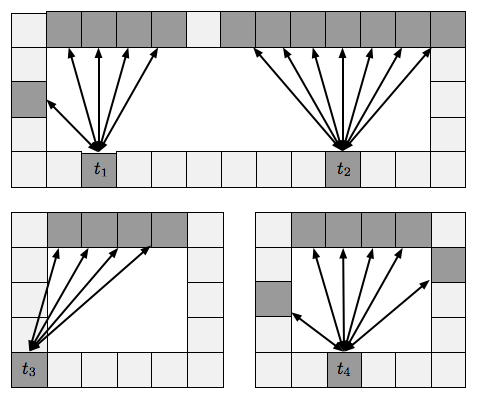
\includegraphics[scale=0.5, trim = 10mm 10mm 10mm 0mm]{diagrams/fan.png}
       \end{center}
	\vspace{-3pt}
       \caption{Some examples.}
       \label{fig-fan}
\end{figure}
